\documentclass[11pt]{article}
\usepackage[letterpaper,margin=0.88in]{geometry}
\usepackage[T1]{fontenc}
\usepackage{lmodern,microtype}
\usepackage{amsmath,amssymb,amsthm}
\usepackage{graphicx,booktabs,tabularx,array,longtable}
\usepackage{xcolor,enumitem,fancyhdr}
\usepackage[numbers,sort&compress]{natbib}
\usepackage{xurl}
\usepackage[colorlinks=true,linkcolor=blue!45!black,citecolor=blue!45!black,urlcolor=blue!45!black]{hyperref}
\usepackage{listings}
\definecolor{navy}{HTML}{17324D}
\definecolor{teal}{HTML}{087F8C}
\lstset{basicstyle=\small\ttfamily,breaklines=true,frame=single,rulecolor=\color{black!18},columns=fullflexible}
\newtheorem{proposition}{Proposition}
\newtheorem{theorem}{Theorem}
\newtheorem{definition}{Definition}
\newcommand{\AtMem}{\textsc{AtMem}}
\newcommand{\code}[1]{\texttt{\small #1}}
\newcolumntype{Y}{>{\raggedright\arraybackslash}X}
\setlength{\emergencystretch}{2em}
\setlength{\parskip}{3pt}
\setlist{nosep,leftmargin=*}
\pagestyle{fancy}\fancyhf{}
\fancyhead[L]{\small\color{navy}Governed Evidence Assembly}
\fancyhead[R]{}
\fancyfoot[C]{\thepage}
\setlength{\headheight}{14pt}
\title{\vspace{-1.1cm}\textbf{Obligation-Guided Evidence Assembly\\and Governed Agent Memory}\\[0.35em]
\large Architecture Evolution, AtMem Benchmark Evidence,\\and Record-to-Audit Integrity}
\author{Javad Taghia\\\small AtMem.Ai Lab\\\small\url{https://github.com/aetna000/atmem}}
\date{10 October 2026}
\begin{document}
\maketitle
\begin{abstract}
Persistent agent memory must recover useful evidence, preserve its authority, and expose when that evidence is incomplete or has been altered. We describe the evolution from AtMem 2.3.7, a governed record and execution-continuity system, to the 2.3.8 source-linked context engine. The new design connects immutable source ranges, typed evidence views, query-derived obligations, independent candidate pools, bounded neighbourhood expansion, coverage-aware context packing, and canonical revalidation at delivery. A separate integrity improvement reconciles current memory records with commitments stored in the audit chain. On a frozen 23-question LongMemEval-V2 development sample, AtMem answers 5 questions; the no-retrieval control answers 1, while a diagnostic condition using evaluator-verified evidence answers 19. On 30 DolphinBench development tasks, AtMem passes 9 tasks and 32 of 97 individual checks. Evidence-removal controls block all 30 tasks, restoration opens all 30 gates, and 29 of 30 paired control cases complete without provider failure. An independent AGMI-maintainer reproduction of AGMI 0.6.3 from the published PyPI wheel reports 8 of 9 storage attacks with the audit chain alone and 9 of 9 with a trusted external checkpoint. We give conditional propositions for evidence coverage, authority confinement, and rollback detection. The contribution is an inspectable integration of retrieval and governance, supported by bounded AtMem benchmark evidence, explicit failure accounting, and a reproducible path toward stronger evaluation.
\end{abstract}
\noindent\textbf{Keywords:} agent memory; evidence coverage; context assembly; memory governance; audit integrity; LongMemEval-V2; DolphinBench.

\section{Introduction}
An agent asked to send a project update needs more than a relevant memory. It needs the correct recipient, the applicable date, the actual project outcome, and any qualification that changes what it is permitted to say. A retrieved passage can mention the project yet omit the outcome. A stored address can be exact yet belong to another workspace. An audit log can be internally valid while the memory table it supposedly explains has been modified. These are different failure modes, and improving nearest-neighbour retrieval alone cannot resolve all of them.

AtMem treats memory as a governed source of context. Its purpose is to preserve reusable evidence and control its delivery across agent hosts. The 2.3.7 release already included scope checks, lifecycle management, context receipts, optional semantic and graph retrieval, and execution continuity. Version 2.3.8 extends this foundation with a new evidence representation and assembly path. It asks not only which memories resemble a request, but which retained source ranges cover the request's declared information needs, whether they fit the context budget, and whether they are still eligible at delivery time.

The practical motivation came from poor results. An early 14-question LongMemEval-V2 run returned an average of 21,539 memory-context tokens and answered no questions correctly. The corresponding no-retrieval arm also answered none. More available text had not produced useful evidence. Development subsequently focused on preserving exact state, retaining action neighbours, separating comparison sides, and avoiding context dominated by transport details or loosely related sources. These changes preceded the final retained development results reported here \citep{history,results}.

The paper makes three contributions. First, it documents an architectural transition using the actual 2.3.7 and 2.3.8 source tags. Second, it formalizes the connection between source evidence, query obligations, packing, and canonical delivery, while identifying where implementation heuristics fall short of the formal model. Third, it reports AtMem utility, control, and integrity evidence with exact configuration boundaries. The reported outcomes are bounded development measurements, not state-of-the-art claims on either complete memory benchmark.

\paragraph{How to read this paper.}
Sections~\ref{sec:architecture}--\ref{sec:mechanisms} explain the system from the architecture down to its data flow. Section~\ref{sec:novelty} identifies the contribution relative to prior systems. Section~\ref{sec:formal} states conditional guarantees. Sections~\ref{sec:methods}--\ref{sec:results} distinguish measurement from interpretation. The appendices map claims to code and list the evidence needed for independent reproduction.

\section{Related Work and Positioning}
\paragraph{Retrieval and persistent memory.}
Retrieval-augmented generation combines parametric generation with external information retrieval \citep{rag}. Generative Agents connects stored observations, reflection, and planning \citep{generative}. MemGPT manages information across memory tiers to work beyond the immediate context window \citep{memgpt}. These establish that external state and selective context construction are substantial prior art. AtMem does not claim to invent external memory, hierarchical memory, or the separation of storage from generation.

\paragraph{Evaluation of memory.}
LoCoMo examines long conversational histories \citep{locomo}; LongMemEval separates indexing, retrieval, and reading and evaluates multiple memory abilities \citep{lme}. DolphinBench tests whether remembered information produces correct tool actions, rather than only verbal recall. The present work uses development subsets of LongMemEval-V2 and DolphinBench. Historical LoCoMo and other AtMem results are not relabelled as 2.3.8 results. Work on long-context utilization also shows that the placement of useful information can affect performance \citep{lost}; that motivates attention to packing without proving our packing method is better.

\paragraph{Integrity and coverage.}
Secure audit logging has long distinguished protected evidence from attacker-controlled storage \citep{audit}. AGMI operationalizes storage-edit tests against memory systems \citep{agmi}. Our contribution here is the specific record-to-audit repair and its reproduction, not a new cryptographic primitive. Likewise, weighted evidence coverage has a classical submodular formulation \citep{submodular}. We use that formulation to explain complementary selection, while making no claim that the complete implementation inherits a classical greedy approximation guarantee.

\section{Architecture: What Changed Between 2.3.7 and 2.3.8}
\label{sec:architecture}
Figure~\ref{fig:architecture} gives the high-level comparison. The release tags resolve to \code{cb1cf0f} for 2.3.7 and \code{267c5b3} for 2.3.8. Architectural statements below are source-derived; benchmark rows retain their own candidate identities.

\begin{figure}[t]
\centering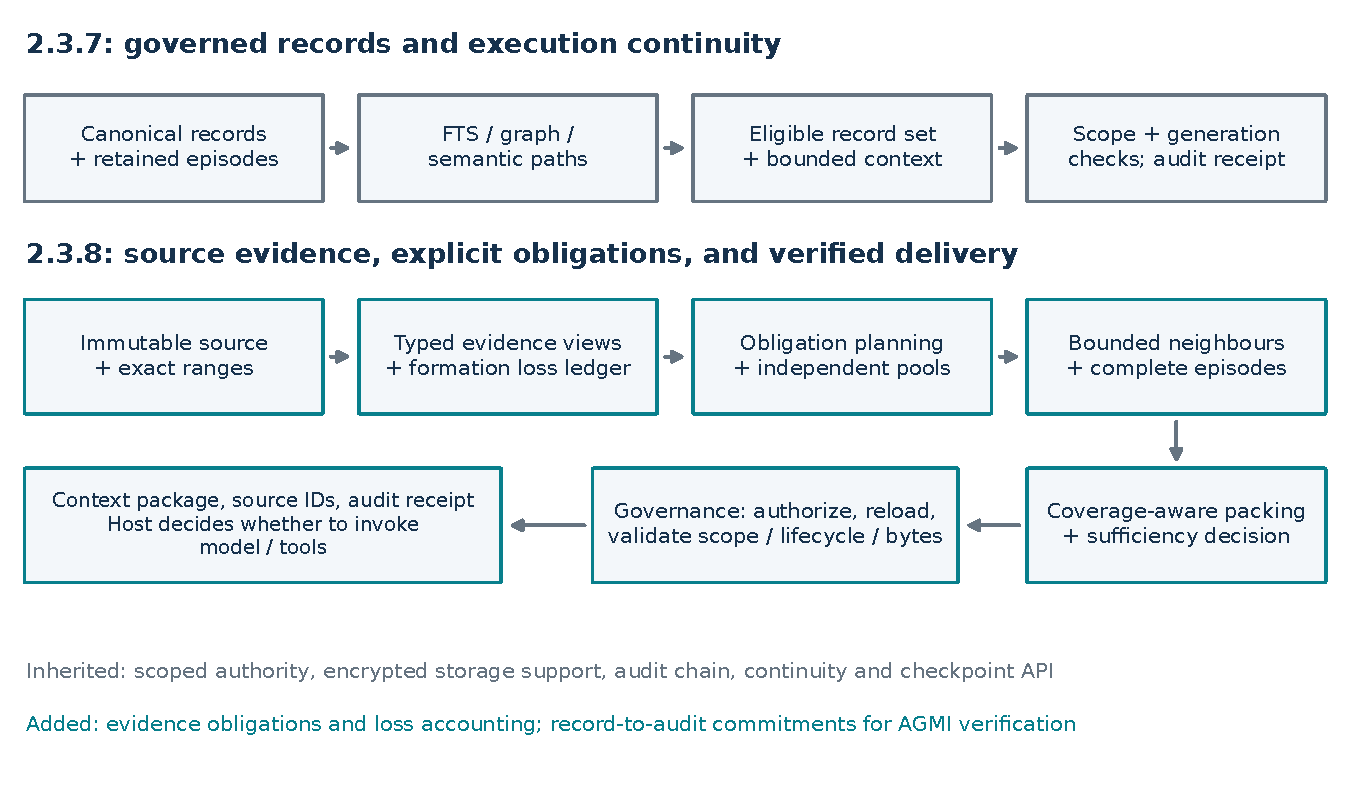
\includegraphics[width=\linewidth]{figures/architecture.pdf}
\caption{Architecture evolution. The upper path summarizes the 2.3.7 record/context interfaces; it does not depict every legacy retrieval path. The lower path adds an explicit source-to-obligation-to-context representation. Scope checks, generation validation, canonical reload, audit receipts, and the checkpoint API have predecessors in 2.3.7.}
\label{fig:architecture}
\end{figure}

\subsection{The 2.3.7 foundation}
The legacy \code{recall()} path retrieves bounded active record candidates through full-text search and can add graph-nominated records. It ranks and blends candidates, filters exclusions, and returns a limited result set. Semantic indexes and other retrieval interfaces also existed. The architecture already separated derived search structures from canonical records.

The \code{prepare\_context\_v1()} interface loaded a candidate set bound to a subject, agent, and workspace. It checked expiry and memory generation, rejected record IDs outside the eligible set, reloaded canonical records, and excluded inactive records. Its serializer appended records within a character budget and recorded accepted IDs and a context digest. Thus, canonical reload and scoped delivery are inherited mechanisms, not claims of novelty for 2.3.8.

Execution continuity addressed another problem: preserving operation identity, receipts, recovery state, and inspection across interrupted work. That infrastructure remains valuable, but continuity does not guarantee that a later query retrieves the complete evidence needed to perform a new task. The new context engine addresses that complementary problem.

\subsection{The 2.3.8 representation and control path}
Version 2.3.8 introduces immutable source episodes and parts, exact ranges within those parts, and rebuildable generations of typed evidence units. A formation receipt distinguishes processing completion from representation completion and records represented and lost ranges. A query plan describes evidence obligations. Retrieval nominates evidence independently across typed pools; bounded expansion adds the local context necessary to interpret a hit. Packing then selects a feasible evidence package rather than truncating a global ranking without regard to missing needs.

The governance service is outside the selection engine. It authorizes a request, gives the engine a manifest, validates the returned IDs and receipt, reloads the exact selection, checks scope, lifecycle and generation, applies the final byte ceiling, and records an audit event. A sufficient selection whose required evidence does not survive packing is downgraded. In this service, non-sufficient status yields an empty model-context string, while the receipt explains the missing or conflicting evidence.

\begin{table}[t]
\centering\small
\begin{tabularx}{\linewidth}{p{.17\linewidth}YY}
\toprule
Dimension & AtMem 2.3.7 & AtMem 2.3.8 addition or change\\\midrule
Canonical basis & Governed records and retained episodes & Immutable source parts and exact ranges supporting typed views\\
Retrieval & Bounded lexical, optional graph and semantic paths & Obligation-specific nominations; typed pools; bounded source neighbours\\
Context assembly & Eligible record serialization under a budget & Complementary coverage and contiguous action episodes; packing-aware status\\
Governance & Scope, expiry, generation, canonical reload, audit & Selection/receipt consistency; exact evidence IDs; final canonical byte check\\
Completeness & Existing relevance and policy decisions & Formation loss receipts; required, covered and missing obligations\\
Integrity & Audit-chain verification and external checkpoint API & Whole-row commitments and reconciliation against live records\\
Hosts & Existing memory and continuity adapters & Reversible native Hermes setup, shadow/active and explicit sharing choices\\\bottomrule
\end{tabularx}
\caption{Verified architectural delta. ``Addition'' does not imply the corresponding general concept was absent from the wider literature.}
\label{tab:delta}
\end{table}

\subsection{Deployment profiles and trust boundaries}
The implementation defines three profiles: \code{legacy-control} for the inherited path, \code{context-fast} for deterministic assembly, and \code{context-navigate} for model-assisted navigation. Navigation requires a model. These are implementation profiles, not three separately scored winners. The final utility results are attached to the recorded candidate arm, not automatically to every profile.

Activation is explicit. Profile state tracks local qualification, active and shadow profiles, generation, and sampling. The default-state function can retain legacy control with a shadow candidate on upgrade, and permits a qualified fast profile for a fresh installation. Hermes setup defaults to an isolated scope and shadow mode. Active recall and cross-agent sharing require explicit choices. Optional AtBot ranking or proposals and AtFlows observations do not grant those components authority to mutate canonical memory \citep{release}.

\section{Technical Mechanisms}
\label{sec:mechanisms}
\subsection{Immutable sources, typed views, and loss accounting}
Let an episode contain ordered source parts $s_1,\ldots,s_m$. We represent a source range as
\[
r=(\mathrm{source},\mathrm{part},a,b,h_s),
\]
where $a,b$ identify a bounded span and $h_s$ binds the retained source. An evidence unit points to one or more such ranges and carries its kind, generation, and retrieval projection. Its identity does not replace the source's authority.

The store rejects reuse of an existing source identity with different source bytes. It creates source parts once and builds views over them. Deterministic formation retains raw ranges and adds evidence shapes for facts, entities, procedures, rules, transitions, gotchas, and premises. Additive extraction can augment these views, but an extracted claim needs grounding and applicable admission checks. Processing every input is insufficient to claim that every relevant fact has become retrievable.

The formation receipt therefore distinguishes \emph{processing complete} from \emph{representation complete}. It records ranges represented, ranges lost or withheld, unit counts, rejections, and storage accounting. A source retained but not represented is a diagnosable formation gap. A source refused by governance is a different outcome from a source silently dropped by an extractor. Neither becomes a successful answer merely because ingestion returned without an exception.

This design also helps remove duplication. Earlier Dolphin diagnostic checkpoints occupied about 1.028 billion bytes; a subsequent compact V3 attempt occupied 245.3 million bytes, about 76.1\% less. That attempt still failed its removal diagnostic because of duplicate nominations and non-atomic targets. The storage improvement is historical diagnostic evidence, not a final matched storage-efficiency result or a claim of superior utility.

\subsection{Query obligations and routing}
A plan contains bounded, explicit information needs derived from the request. Examples include subject--relation--value, ordered steps, before--action--after, premise checking, and condition--action evidence. A user requesting a comparison needs both sides; a user asking what changed needs evidence for the transition, not just two nearby timestamps.

The planner is concrete heuristic software. It uses request clauses, lexical cues, identifiers, dates, and action-content facets. It strips known host scaffolding so that a tool schema does not become a fictitious memory obligation. It bounds decomposition; for example, the inspected clause splitter retains at most four distinct clauses. These choices improve tractability but can miss implicit requirements.

For addressed actions, the planner separates content needs from the delivery address. Otherwise an exact email address can dominate retrieval even when the needed outcome appears in a different source episode. Content facets remain nominations rather than new mandatory obligations. This distinction matters: adding every query expansion as a required fact would cause unnecessary blocking.

No claim of general semantic understanding follows from this planner. The source includes explicit workflow patterns, including ServiceNow Problem/Incident distinctions in option-field packing. These are application-specific heuristics introduced during development. They consume request and source text, rather than evaluator answers at runtime, but still create development adaptation and must be evaluated on unseen environments.

\subsection{Independent pools and bounded evidence expansion}
The V3 pool definitions include raw state, transition, fact, entity, procedure, rule, gotcha, and premise. The inspected default candidate budget permits 32 nominations per pool and 200 total units. Candidate limits are separate from the delivered-context budget. More nomination breadth does not imply permission to deliver more bytes.

The inspected fast path uses indexed lexical candidates and intent-specific ordering and grounding. Other product retrieval facilities include semantic and graph paths. The release description names all of these capabilities; that description is not evidence that every signal was active in the final benchmark arm. We therefore avoid assigning measured gains to a neural reranker, graph algorithm, or learned embedding that was not isolated in the run.

Once a head candidate is found, bounded source neighbours recover the condition, action, outcome, value tail, or identity field that makes it useful. Exact date and identifier nominations help select the correct episode. Indirect references to the usual recipient can retain an adjacent source-backed address. Selected sources may contribute related ranges without each range independently outranking every unrelated candidate.

Consider an illustrative request: ``Email the integration contact the final outcome of the September review and explain the remaining restriction.'' Retrieving the contact directory alone finds the destination but not the outcome. Retrieving a review summary without the restriction produces an incomplete action. AtMem's intended behaviour is to cover recipient, outcome, and restriction, preserve their provenance, and block or withhold context if its required evidence is missing. This example illustrates the mechanism; it is not a fabricated benchmark trace.

\subsection{Complementary packing and episode continuity}
The packer prioritizes required evidence, complementary field coverage, and source groups relevant to addressed actions. Within a selected action episode it preserves source order so that trigger, action, result, and qualification remain interpretable together. This addresses a failure in which the right source was retrieved but fragmented around unrelated recipients or caveats.

One implementation helper greedily prefers new option-field coverage per byte. Another orders action source groups and preserves their contiguous ranges. The implementation is consequently more specific than a generic ``top-$k$'' selector and less general than a globally optimal constrained coverage solver. The service subsequently uses the IDs that actually survived packing. It does not reload excluded candidates and accidentally reintroduce text that was deliberately removed to satisfy the budget.

\begin{figure}[t]
\centering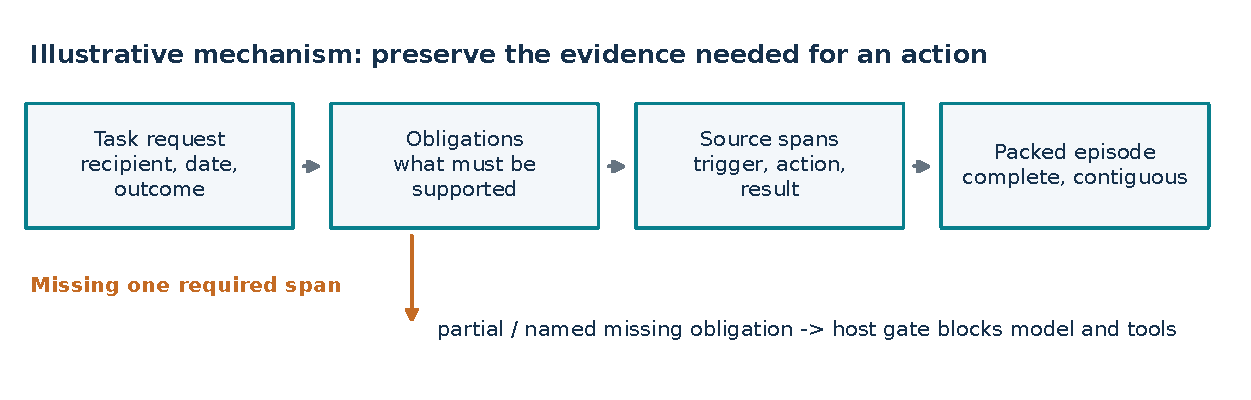
\includegraphics[width=\linewidth]{figures/evidence_flow.pdf}
\caption{A conceptual request-to-evidence path. Runtime obligations come from the request; evaluator requirement annotations are reserved for diagnostics. A host must explicitly enforce the resulting status for missing evidence to prevent model or tool invocation.}
\label{fig:evidence}
\end{figure}

\subsection{Sufficiency is a typed decision, not a calibrated probability}
The actual status vocabulary includes \code{sufficient}, \code{partial}, \code{conflicted}, \code{contradicted}, \code{stale}, \code{not\_found\_within\_budget}, and \code{withheld\_by\_policy}. Required obligations are covered by matched evidence IDs, minus obligations withheld because their source episode is incomplete. Missing required IDs prevent a sufficient result.

Conflict and contradiction detection are bounded heuristics. The inspected code checks negative language for premise obligations and distinct numeric or channel values for certain approval-sensitive questions, with correction cues. This does not establish general contradiction resolution. A receipt saying ``sufficient'' means the implemented coverage rule accepted the declared obligations; it does not mathematically certify that an arbitrary natural-language answer is true.

Packing can invalidate sufficiency: retrieving complete evidence does not help if required material is excluded from the final package. The service downgrades a sufficient decision when packing is incomplete, records \code{context\_budget\_exhausted}, and propagates the actual selected IDs. This coupling between the decision and the delivered package is a central integration contribution.

\subsection{Canonical revalidation and host responsibility}
The selection engine operates under an authorized manifest. The governance service rejects duplicate IDs, unauthorized selections, sufficiency evidence outside the selection, mismatch between plan obligations and the receipt, and undeclared external egress. It reloads selected canonical evidence and verifies exact order, scope, generation, and active lifecycle. The context digest and audit event identify what the service prepared.

This protects the context boundary against an erroneous or overreaching selector under the stated authorization assumptions. It does not imply that a host will obey the receipt, that arbitrary tools cannot bypass the host adapter, or that earlier context already observed by a model can be erased. The Dolphin adapter's pre-action gate is one explicit consumer of the status. A different integration needs its own enforcement and observation tests.

\section{What Is Novel, and What Explains the Observed Progress?}
\label{sec:novelty}
The simplest description of the proposed contribution is \emph{evidence obligations connected to governed delivery}. It is an engineering composition with inspectable contracts. It is not a claim to have invented typed memory, source attribution, graph retrieval, or a hash chain.

\begin{table}[t]
\centering\small
\begin{tabularx}{\linewidth}{p{.24\linewidth}Y}
\toprule
Boundary & AtMem 2.3.8 contract\\\midrule
Stored evidence & Immutable source episodes, exact ranges, derived typed units, and formation-loss receipts\\
Query interpretation & Bounded obligations for facts, transitions, procedures, premises, conditions, actions, and outcomes\\
Candidate formation & Independent typed pools, grounded heads, exact-value routes, and bounded source neighbours\\
Context assembly & Complementary coverage, contiguous action episodes, byte-aware packing, and post-packing sufficiency\\
Governed delivery & Authorized manifest, canonical reload, scope, generation, lifecycle, selected IDs, byte ceiling, and audit receipt\\
Integrity & Whole-row commitments, live-record reconciliation, and optional trusted rollback checkpoint\\\bottomrule
\end{tabularx}
\caption{The integrated AtMem 2.3.8 evidence and governance contract.}
\label{tab:system-contract}
\end{table}

\paragraph{Novel integration relative to the earlier AtMem.}
The old context boundary proved eligibility of a selected record set. The new path adds an explicit explanation of what information is needed, which source ranges represent it, which parts are missing, and whether that support survived the packing budget. It extends existing canonical revalidation to typed evidence and selection receipts. This allows downstream hosts to distinguish evidence absence from a retrieval score below a threshold.

\paragraph{Why the integration matters.}
The system does not treat a high retrieval score as proof that a request is answerable. It distinguishes retained source from represented evidence, candidate evidence from packed evidence, and packed evidence from authorized delivery. Each transition can expose a loss or rejection. This makes failures inspectable at the boundary where they occur instead of collapsing them into one final answer score.

\paragraph{Mechanism hypotheses, stated precisely.}
The development work suggests three hypotheses: preserving exact values and workflow identity increases availability of answer-bearing evidence; bounded expansion recovers necessary conditions and outcomes; and packing complete episodes reduces reader omissions. Historical diagnoses and code changes support these as explanations worth testing. No completed factorial ablation assigns an independent effect size to any of them. Governance and integrity address reliability dimensions that were not isolated as causes of the clean-data accuracy gains.

\paragraph{The claim that can be defended.}
AtMem 2.3.8 implements the complete source-to-obligation-to-delivery path and produces measurable results on two development samples, paired evidence-removal controls, and a pinned integrity suite. Assigning causal credit to individual mechanisms requires held-out evaluation and component ablations. We therefore present the integration and its reproducible research questions without translating development progress into a universal performance claim.

\section{Formal Model and Conditional Guarantees}
\label{sec:formal}
The following statements explain the architecture. They are mathematical results under explicit assumptions, not formal verification of the Python implementation or proofs of benchmark superiority.

\subsection{Authorized evidence and coverage}
Let $U$ be the retained evidence units, $q$ a request, and $A(q)\subseteq U$ the units allowed by the current authority, lifecycle and generation checks. Let $O(q)=\{o_1,\ldots,o_m\}$ be declared obligations. Define $g(u,o)\in\{0,1\}$ as a fixed evidence-grounding relation. For nonnegative weights $w_o$, define
\begin{equation}
 F(P)=\sum_{o\in O(q)}w_o\,\mathbf{1}\!\left[\exists u\in P:g(u,o)=1\right],\qquad P\subseteq A(q).
 \label{eq:coverage}
\end{equation}
Packing seeks high coverage under a context cost $c(P)\leq B$, subject to required obligations and eligibility. This objective is an explanatory abstraction. Actual coverage labels are heuristic, costs include serialization overhead, and source grouping changes which candidate combinations are feasible.

\begin{proposition}[Diminishing returns of fixed obligation coverage]
For fixed $A(q)$ and $g$, $F$ is monotone and submodular. If every unit has equal cost and feasibility is only $|P|\leq k$, classical greedy coverage obtains at least $(1-1/e)$ of the optimal coverage.
\end{proposition}
\begin{proof}
Adding a unit cannot remove a covered obligation, proving monotonicity. For $P\subseteq Q$, the obligations newly covered by a unit outside $Q$ form a subset of those it newly covers outside $P$. Nonnegative weights preserve this inequality, proving diminishing returns. The equal-cost cardinality case then satisfies the assumptions of the classical greedy bound \citep{submodular}.
\end{proof}
The production packer includes unequal byte costs, mandatory heads, grouped sources and heuristic ordering. We explicitly do not transfer the $1-1/e$ guarantee to it. If support requires a conjunction of several units, the binary per-unit relation is also insufficient; a hyperedge or structured-obligation model is needed, and the resulting objective need not be submodular.

\begin{proposition}[Conditional authority confinement]
Assume the authorizer returns exactly the permissible IDs for request $q$; canonical reload and lifecycle checks are sound; and no unauthorized change occurs between validation and serialization. If preparation returns successfully and serializes only its reloaded selected units, every delivered unit lies in $A(q)$.
\end{proposition}
\begin{proof}
The service first checks selection containment in the authorized manifest. Reload must return the exact selected IDs and order. It then checks each unit's scope, generation, and lifecycle. Serialization uses only those units. Any delivered unit outside $A(q)$ would contradict at least one assumed sound check.
\end{proof}
This proves an output-membership property, not timing noninterference, correct authorizer policy, or protection against a host bypass. Transaction and concurrency behaviour must preserve the stated assumptions.

\begin{proposition}[No loss of declared support at a correctly enforced packing boundary]
Assume $O(q)$ contains all required obligations, $g$ is sound, and the emitted sufficient status is permitted only if every $o\in O(q)$ is supported by the final packed set $P$. Then sufficient delivery entails declared evidence coverage within the budget.
\end{proposition}
\begin{proof}
The status precondition gives a supporting unit in $P$ for every required obligation. The packer and final serializer check $c(P)\leq B$. Both claims follow directly. They do not imply that the reader interprets the evidence correctly.
\end{proof}
The assumptions are deliberately strong. The implemented planner may omit needs, grounding may be inaccurate, and contradiction handling is incomplete. Removal controls test selected instances of this boundary; they do not establish universal semantic sufficiency.

\subsection{Integrity binding and rollback}
Let $\phi(r)$ be a canonical projection of a memory record and $d_r=H(\phi(r))$ its committed digest. The projection includes identity, subject, content, source fields, trust tier, time, confidence, scope, status, supersession, fact key, and raw payload. A protected audit event commits to $d_r$. Verification must reconcile live records against events, rather than checking only links between events.

\begin{proposition}[Detection for an unchanged, committed record]
Assume a trusted audit commitment $d_r$ cannot be replaced, $H$ is second-preimage resistant, the verifier checks the live record against $d_r$, and no authorized lifecycle exemption applies. Changing any field included in $\phi(r)$ is detected except with negligible cryptographic probability.
\end{proposition}
\begin{proof}
An altered projection $\phi(r')\neq\phi(r)$ can pass only if $H(\phi(r'))=d_r$. This is a second preimage under the assumptions. Removing a required committed row is detected by existence reconciliation rather than a hash comparison.
\end{proof}
This statement is intentionally narrower than ``all memory is tamper-proof.'' The inspected implementation leaves legacy records without commitments identifiable as legacy and skips records marked legitimately changed by certain lifecycle events. Integrity coverage for those paths must be audited separately. A valid digest also cannot establish whether originally admitted text was factually correct.

\begin{theorem}[Whole-store rollback cannot be recognized from the rolled-back store alone]
Suppose a verifier has no trusted state outside a writable store. If it accepts a legitimate earlier snapshot $S_t$, it cannot always reject the identical snapshot after an attacker replaces a later store $S_{t+1}$ with $S_t$.
\end{theorem}
\begin{proof}
Compare two worlds: the store legitimately remains at $S_t$, and the store advanced to $S_{t+1}$ before being restored to $S_t$. The verifier receives identical trusted inputs in both worlds. Its output distribution is therefore identical. Always accepting the legitimate old state and always rejecting the rollback is impossible without another trusted distinguishing input.
\end{proof}
An external checkpoint containing a later chain position and hash provides such an input. Its freshness bounds the protected interval, and its storage must be outside the attacker's rollback domain. Merely hashing a checkpoint stored beside the database does not satisfy this requirement.

\section{Experimental Method and Configuration Audit}
\label{sec:methods}
\subsection{Evidence scope and provenance}
This paper analyzes retained reports and source; it does not run new paid experiments. The compact reports are available in the repository, while the heavy raw histories and run archives are referenced on an external volume that was not mounted during manuscript preparation. Counts are therefore verified against the retained compact records, not independently recomputed from every raw trajectory.

The stable architecture is read at tag \code{v2.3.8}. The utility measurements were made on development candidates, including artifacts retaining the \code{2.3.8b6} version. The final Dolphin candidate is \code{b97d35e}. The vendor AGMI candidate wheel was built from \code{fdc63de}; the AGMI maintainer independently reproduced its outcomes from the published PyPI wheel, whose installed package matches tag \code{v2.3.8}. Relative to \code{fdc63de}, the package differs only in a compatibility comment and tested OpenClaw version string. A single stable tag was not rerun across all utility rows. We use ``2.3.8 candidate'' for utility and keep AGMI's published 2.3.8 identity explicit.

\subsection{Samples and metric definitions}
LongMemEval-V2 uses 23 of 451 questions, or 5.10\%. The sample retains all 14 historical pilot IDs and adds nine IDs selected by a salted hash from the remaining development partition. It is thus a nested development sample, not a fresh random test. DolphinBench uses 30 of 600 tasks, exactly 5\%, across the three personas. Historical ingestion processed all 13,539 released sessions; the small task fraction does not mean only 5\% of the history was ingested.

LongMem accuracy is $\sum_i y_i/n$, with failed system executions retained in $n$. Dolphin task success requires the task's complete grading outcome; individual check success is a separate metric. The 97 checks are clustered within 30 tasks and are not 97 independent experimental units. AGMI reports detection outcomes for nine fixed attack classes; these are conformance cases, not an estimated probability of detecting arbitrary attacks.

\subsection{Versions, models and evidence boundaries}
\begin{table}[t]
\centering\small
\begin{tabularx}{\linewidth}{p{.23\linewidth}Y}
\toprule
Component & Frozen identity / configuration\\\midrule
AtMem stable architecture & 2.3.8, commit \code{267c5b3}; 2.3.7 comparison at \code{cb1cf0f}\\
AtMem utility candidates & Historical 2.3.8b6 identities retained; final Dolphin code \code{b97d35e}\\
Reader / agent & Qwen/Qwen3.5-9B, revision \code{c202236235762e1c871ad0ccb60c8ee5ba337b9a}\\
Judge route & \code{gpt-5.2-2025-12-11}, medium reasoning, where semantic grading applies\\
LongMem embeddings & Local \code{atmem/hash-bow-768-v1} route; signed token hashing, not a learned semantic encoder\\
Dolphin reader route & Hugging Face inference providers with the recorded Qwen model identity\\
AGMI & 0.6.3, commit \code{115493a41a7b41952f92ec07e1ea0932926e194f}\\\bottomrule
\end{tabularx}
\caption{AtMem configuration and frozen identities used by the reported evidence.}
\label{tab:config}
\end{table}

The final Dolphin reader route used Hugging Face inference providers; LongMem used the recorded RunPod reader route. Shared model identity does not imply shared provider execution across the two benchmarks. The utility measurements were produced by development candidates rather than one stable artifact rerun across every row. A fresh environment lock, installed-artifact receipt, checkpoint digest, provider settings, prompts, case traces, and grading outputs remain necessary for exact independent reproduction.

\subsection{Controls and failure accounting}
LongMem includes no-retrieval and evaluator-verified evidence controls. The latter supplies privileged supporting evidence to the same reader; it is a diagnostic reference for that controlled input, not a deployable result or a universal accuracy ceiling. Its success indicates opportunity to improve evidence delivery or use, but not which pipeline stage is solely responsible.

Dolphin removal controls remove evaluator-selected evidence after formation, then require a named missing obligation, no model invocation, and zero tool calls. Restoration is a positive control: an agent that always blocks must not receive a safety success. The recorded removal result is 30/30 and restored gate opening is 30/30; paired removal-and-positive controls are 29/30, with one provider failure. These controls belong to their recorded development attempt and are not silently relabelled as a fresh final-candidate control run.

\section{Results and Their Statistical Meaning}
\label{sec:results}
\begin{table}[t]
\centering
\begin{tabular}{lrr}
\toprule
Metric & Count & Rate\\\midrule
LongMem correct & 5/23 & 21.7\%\\
LongMem no-retrieval control & 1/23 & 4.3\%\\
LongMem evaluator-verified evidence diagnostic & 19/23 & 82.6\%\\
LongMem system failures & 6/23 & 26.1\%\\
Dolphin tasks passed & 9/30 & 30.0\%\\
Dolphin checks passed & 32/97 & 33.0\%\\
Dolphin evidence-removal blocks & 30/30 & 100\%\\
Dolphin restoration gate openings & 30/30 & 100\%\\
Dolphin paired controls completed & 29/30 & 96.7\%\\\bottomrule
\end{tabular}
\caption{AtMem utility and control evidence from the frozen development reports. Counts retain system and provider failures in their stated denominators.}
\label{tab:results}
\end{table}

\subsection{Observed AtMem outcomes}
AtMem answers 5 of 23 LongMem questions and passes 9 of 30 Dolphin tasks, including 32 of 97 individual checks. These are descriptive development outcomes. They show that the source-linked context path can deliver answer-bearing evidence and support successful tool trajectories in selected cases; they do not estimate population performance on the complete benchmarks.

Absolute performance is still weak. AtMem fails to answer 18 of 23 LongMem questions correctly and does not fully pass 21 of 30 Dolphin tasks. Six LongMem cases are classified as system failures: three reader finalization failures at the 20,000-token completion cap and three governance rejections described in the report as outside the frozen selection. That wording needs case-level reconciliation before allocating terminal blame. All six remain in the denominator; we do not silently remove them to increase accuracy.

\subsection{Evidence versus no memory}
The no-retrieval LongMem arm answers 1/23, while evaluator-verified evidence yields 19/23. AtMem product context obtains 5/23. Thus product context has four more observed successes than the no-memory control, and a 14-question aggregate gap remains to the verified-evidence condition. These are aggregate differences, not claims that exactly four specific cases were rescued or that precisely 14 retrieval errors occurred. Case overlaps and controlled stage ledgers are needed for that attribution.

\subsection{Control interpretation}
The Dolphin removal control asks whether the governance path recognizes a deliberately created evidence gap. All 30 removal cases produced the required block, and all 30 restored cases opened the gate. The combined paired procedure completed in 29 cases, with one provider failure. This result tests responsiveness to a named missing obligation; it does not prove that the planner identifies every obligation in arbitrary requests or that every opened gate produces a correct action.

The development samples were repeatedly inspected while the implementation changed. Population confidence intervals and paired generalization claims would therefore overstate what the retained counts establish. The appropriate next inference comes from untouched tasks and symmetric repetitions under a frozen artifact.

\subsection{Engineering trajectory, not causal ablation}
The early LongMem pilot's 0/14 and final 5/23 use different sample sizes and evolving code; they cannot be subtracted as a clean treatment effect. A seven-question diagnostic briefly reached 4/7 after changing evidence projection and reader limits, followed by 3/7 on another confirmation. The retained negative results show why a peak intermediate score should not be selected as the release score \citep{history}.

For the fixed Dolphin development sample, the earliest retained AtMem result is 2/30 tasks and 15/97 checks. The final result is 9/30 and 32/97 following action-evidence neighbourhood and identity-routing work. This association motivates the mechanism hypotheses, but model/provider effects, repeated attempts, and multiple code changes remain confounded. A valid ablation would freeze the same artifact, formation checkpoint, reader, provider, budgets, and repetition policy while removing one mechanism at a time.

\section{AGMI: From an Intact Audit Chain to Verifiable Memory Records}
\label{sec:agmi}
\subsection{The exposed gap and the repair}
The pinned upstream 2.3.7 AGMI result reports none of nine attacks for the chain-only profile and one of nine for the external-checkpoint profile. This did not mean AtMem had no audit chain. It meant record-level edits could change the table read by the agent without invalidating the independently verified audit events. The checkpoint already exposed the whole-store rollback case. The fundamental repair in 2.3.8 is binding the live record projection to an audit commitment and reconciling the two.

Creation and quarantine events can carry a whole-row integrity digest. Verification collects commitments, known record IDs, and legitimate lifecycle changes, compares eligible live rows to their commitments, reports missing committed rows, and identifies non-tombstoned records with no recognized creation event. Checking content alone would miss attacks on ownership, trust, ordering-related metadata, or lifecycle state; the explicit projection broadens the bound fields.

\begin{figure}[t]
\centering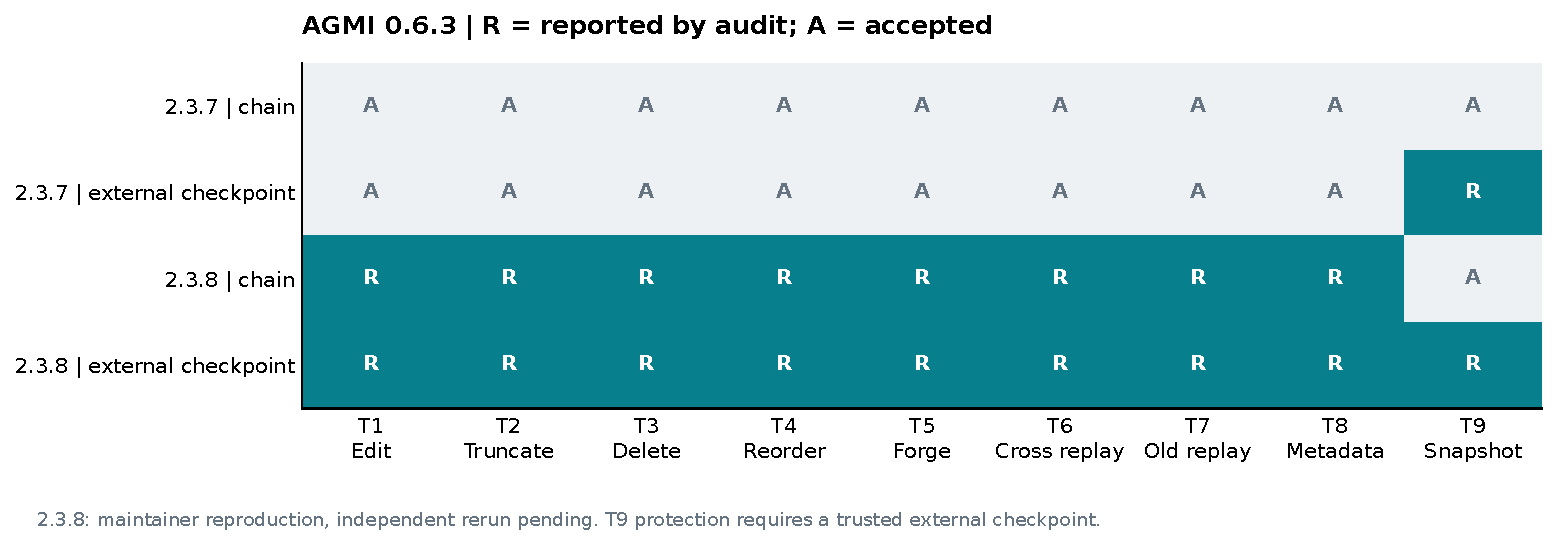
\includegraphics[width=\linewidth]{figures/integrity.pdf}
\caption{AGMI attack-class outcomes. ``Reported'' means the audit path reports a problem, not that every ordinary read API independently rejects it. The 2.3.8 rows were independently reproduced by the AGMI maintainer from the published PyPI wheel on Linux and macOS; the 2.3.7 rows are the retained upstream baseline.}
\label{fig:integrity}
\end{figure}

\subsection{Measured result and operational interpretation}
The installed 2.3.8 wheel reports T1--T8 under both profiles: tampering, truncation, middle deletion, reordering, forging, cross-context replay, record rollback replay, and metadata tampering. T9, whole-store snapshot rollback, is accepted without an external checkpoint and reported with one. The result is 8/9 and 9/9 respectively.

The report records \emph{reported} verdicts. We therefore claim audit detection, not universal blocking before every read. The checkpoint must remain trusted, outside the writable store, and be updated after genuine writes to protect those writes against rollback. Its mere existence does not protect changes made after the latest anchor.

Legacy stores and legitimate mutations are explicit limits. The inspected verifier enables whole-row reconciliation only when a commitment exists. It also skips records identified as legitimately changed by specified events. A malicious edit after such a transition may require a refreshed commitment and additional checks; the fresh seeded AGMI cases do not prove complete lifecycle coverage. This manuscript documents that boundary rather than using a 9/9 result as evidence that every persisted AtMem table or mutation path is protected.

\subsection{How integrity contributes to useful memory}
Integrity improves the basis on which a memory can be trusted for reuse. A source-backed recipient, date, or permission is useful only if the stored evidence still corresponds to the authorized history. Record reconciliation detects a class of silent substitutions, and an external checkpoint detects an otherwise indistinguishable old store. These support reconstruction and investigation of why a memory was supplied.

They do not establish that the evidence was true at admission, eliminate prompt injection, or improve a reader's answer on their own. The clean-data utility benchmarks contain no controlled integrity intervention. Accordingly, we claim complementary utility and integrity evidence, not that AGMI success caused the LongMem or Dolphin score increase. An appropriate future experiment would measure action correctness before and after deliberate storage attacks, with verification enforcement on and off.

\section{Discussion, Limitations, and Research Agenda}
\subsection{Why the architecture merits continued investment}
The durable value proposition is an inspectable contract across source retention, context selection, authority, and host delivery. The retrieval engine can change without transferring canonical authority to a model or index. Source ranges make it possible to investigate selection and rebuild derived views. Missing-obligation receipts let a host choose a controlled response instead of treating a search hit as sufficient permission to act. Record commitments make part of the persisted history auditable against the live state.

These properties offer a credible reason for AtMem to compete alongside established memory systems. They are architectural reasons to invest in the system, not a prediction that the product must succeed. A deployment must still demonstrate acceptable latency, storage overhead, recall, operational reliability and host support on its own workload.

\subsection{Threats to validity}
The central limitation is development adaptation. The LongMem sample contains earlier inspected questions, and the Dolphin sample was reused while adding rules and selecting candidate code. Runtime separation from evaluator labels is necessary but does not remove tuning to a benchmark's vocabulary or failure modes. Application-specific branches in the packer are especially important to disclose.

Representation and runtime choices are another limitation. The LongMem route uses deterministic hash embeddings rather than a modern learned encoder, while benchmark execution depends on recorded reader, judge, provider, and completion settings. These choices constrain the measured AtMem configuration and prevent treating the counts as a complete characterization of the architecture's achievable performance.

Operational failures confound quality. The LongMem system-failure count is substantial. The final Dolphin run has no recorded system failures, but stochastic readers and reused development artifacts still require symmetric repeated trials. The observed task count is small, and checks within a task are dependent. No uncertainty band should disguise these facts.

Formal claims also have limits. The planner is not complete, grounding is not a sound general theorem prover, and the source does not establish constant-time or complete cross-scope noninterference. The integrity theorem assumes a trusted commitment; lifecycle exemptions and legacy rows need additional qualification. A nine-case suite cannot justify a complete security claim. Finally, independent raw-result regeneration was not possible from the mounted evidence during manuscript preparation.

\subsection{Experiments needed next}
A stronger submission should freeze untouched confirmation IDs, pin every installed artifact, and repeat AtMem evaluation under both the current deterministic profile and a documented learned-embedding profile. It should preserve the current route as an ablation, repeat reader and provider calls symmetrically, and publish case-level stage ledgers for formation, retrieval, packing, governance, model finalization, and grading.

Component ablations should remove typed formation, obligation routing, source-neighbour expansion, episode grouping, and sufficiency gating separately. The endpoint should include evidence-set recall, exact-value retention, action success, false blocking, and reader finalization. Ablation results must retain errors and failed admissions. A repeated-trial paired analysis on held-out tasks can then test which components contribute beyond chance and which merely fit inspected examples.

Governance qualification should examine concurrent invalidation, cross-scope selection, deletion propagation, expired evidence, host bypass, and the difference between prepared and actually delivered context. Integrity qualification should include legitimate updates followed by tampering, pre-upgrade rows, all relevant storage surfaces, stale checkpoints, and automatic enforcement modes. These extend the current record-level AGMI evidence into a broader operational argument.

\section{Conclusion}
AtMem 2.3.8 advances the project from governed record selection toward explicit evidence assembly: retain source ranges, form typed views, state the information required, gather complementary support, preserve it within the budget, and validate the final selection before delivery. The integration extends a substantial 2.3.7 governance foundation. Whole-row audit commitments separately address the memory-table gap exposed by AGMI.

The AtMem candidate answers 5 of 23 questions on the retained LongMem development sample and passes 9 of 30 Dolphin tasks, with complete removal and restoration gate responses in the recorded controls. Absolute accuracy remains low, six LongMem cases are system failures, and the samples cannot support generalization claims. The constructive research claim is nevertheless concrete: useful memory and accountable memory can be developed within one architecture, with failures exposed through source, obligation, delivery, control, and integrity evidence. Establishing the contribution of each mechanism on held-out tasks remains an empirical task.

\paragraph{Disclosure and authorship.}
This is an AtMem-maintainer technical draft. Text, source inspection, formal exposition, and figure preparation were assisted by an AI coding assistant. The reported benchmark measurements predate this manuscript; no new benchmark scores were generated for it. Author review and independent reproduction are required before presenting it as a finalized scientific submission. No independent peer review or arXiv acceptance is implied.

\bibliographystyle{plainnat}
\bibliography{references}

\appendix
\section{Reproducibility and Source-to-Claim Map}
The supplied source package includes the LaTeX manuscript, bibliography, original vector figures and PNG exports, a figure-generation script, descriptive-statistics calculations, and compact repository evidence. Compile with \code{tectonic atmem-2.3.8.tex}; the README gives the exact commands. The bundle contains no API keys, private histories, or fabricated raw cases.

\begin{longtable}{>{\raggedright\arraybackslash}p{.29\linewidth}>{\raggedright\arraybackslash}p{.65\linewidth}}
\toprule Claim / mechanism & Source location at tag \code{v2.3.8}, unless noted\\\midrule
\endhead
Legacy scoped serialization & \path{atmem/memory.py}, \code{prepare\_context\_v1}; also inspect tag \code{v2.3.7}\\
Legacy audit-only comparison & \path{atmem/memory.py}, \code{verify} at \code{v2.3.7}\\
Typed contracts and loss receipts & \path{atmem/context_engine/contracts.py} and \path{formation.py} in that directory\\
Query obligations and facets & \path{atmem/context_engine/planner.py}\\
Candidate budgets and neighbours & \path{atmem/context_engine/pools.py}; \path{atmem/context_engine/retrieval.py}\\
Complementary / episode packing & \path{atmem/context_engine/packing.py}\\
Status and final validation & \path{atmem/context_engine/sufficiency.py}; \path{atmem/context_engine/service.py}\\
Audit binding and exceptions & \path{atmem/memory.py}, \code{\_record\_integrity\_sha256}, \code{\_verify\_record\_integrity}, \code{verify}\\
LongMem formation / embeddings & \path{research/production_benchmarks/prepare_longmem_memories.py}; \path{local_embedding_proxy.py} in that directory\\
Frozen utility summary & \path{benchmarks/retrieval_quality/baselines/five-percent-results-20261010.json}\\
Final Dolphin summary & \path{benchmarks/retrieval_quality/baselines/dolphinbench-final-b97d35e.json}\\
AGMI installed artifact & \path{benchmarks/retrieval_quality/baselines/agmi-2.3.8-20261010.json}\\\bottomrule
\end{longtable}

The benchmark summary's top-level candidate identity is not a per-arm environment lock. The paper therefore does not infer an exact LongMem source commit from the final Dolphin commit. Similarly, the Dolphin summary contains a candidate-artifact hash and the report lists a wheel hash; these are retained as named fields without assuming they are the same object. Independent reproduction needs the underlying per-arm installed-identity receipt, dependency lock, checkpoint digest, provider settings, prompts, case traces and grading outputs.

\clearpage
\section{Evidence Inventory and Identity Boundaries}
\begin{small}
\begin{longtable}{>{\raggedright\arraybackslash}p{.26\linewidth}>{\raggedright\arraybackslash}p{.68\linewidth}}
\toprule Artifact & Recorded identity\\\midrule
\endhead
Stable architecture commit & \path{267c5b3ac08e8cac26dfee13c6eac2842d4bb876}\\
2.3.7 source commit & \path{cb1cf0fc6e3e12dd0a52140bc0eda4797d2e887b}\\
Final Dolphin candidate & \path{b97d35e1df7ee6ef435928bafb8189ac99a1856d}\\
AGMI vendor-candidate source & \path{fdc63de4b5ced0029f2717ee542b9600730ce3fd}\\
AGMI independent confirmation & \href{https://github.com/tech4biz-yasha/agent-memory-integrity/pull/7}{AGMI PR 7}\\
LongMem aggregate SHA-256 & \path{89c800219cfab38b34cfc406d764919b49c24b550827a30414cb49fb4c247fd8}\\
Verified-evidence control SHA-256 & \path{26ba0c7d60b950ec0a5435813b6c7316a0b0badcd9050478b1ff0f262d3bddd6}\\
Final Dolphin AtMem evaluation SHA-256 & \path{aa5242c509f4748a4ab067a56e8bedda3787abfdbc6e0df0ce63b80e936fd358}\\
AGMI vendor-candidate wheel SHA-256 & \path{61cf17963177bd7e9c6a5e9fe18a3be30356cc0b2d4d6d373b215a9fe12266dd}\\
AGMI published PyPI wheel SHA-256 & \path{05ca2c579be1af55de1da056ae257062417831b2e8eb4f2fda2a6413ba3ee923}\\
AGMI runner output SHA-256 & \path{5498bedba335d6c7f40846e17e13413e22d25c298675aa34536c80315f60cceb}\\\bottomrule
\end{longtable}
\end{small}
Hashes identify retained artifacts; they do not prove correctness of their contents. This paper checks the compact inventory and code correspondence but does not claim access to all hashed raw files.

\section{Algorithmic Specification for Review}
The following pseudocode summarizes the intended boundary. It is an explanatory specification, not a line-for-line implementation or a claim that the grounding relation is complete.
\begin{lstlisting}
prepare_context(request):
    manifest = authorize(request.scope, request.generation)
    plan = derive_bounded_obligations(request.query)
    candidates = nominate_by_obligation_and_pool(plan, manifest)
    candidates = deduplicate_and_expand_source_neighbours(candidates)
    decision = assess_declared_evidence_coverage(plan, candidates)
    packed = pack_complementary_evidence(candidates, request.budget)
    if required_support_lost(decision, packed):
        decision = partial(reason="context_budget_exhausted")
    assert packed.ids subset_of manifest.authorized_ids
    canonical = reload_exact_selection(packed.ids)
    assert scopes_generations_lifecycles_match(canonical, request)
    context = serialize(canonical) if decision.sufficient else ""
    assert utf8_bytes(context) <= request.context_byte_budget
    receipt = audit(request, plan, decision, packed.ids, hash(context))
    return context, decision, receipt
\end{lstlisting}

\clearpage
\section{An Ablation Matrix That Would Test the Novelty Claim}
\begin{table}[!ht]
\centering\small
\begin{tabularx}{\linewidth}{p{.25\linewidth}YY}
\toprule Intervention & Hold fixed & Question answered\\\midrule
Remove typed views & Sources, learned embedder, reader, byte budget & Do evidence shapes help beyond raw source retrieval?\\
Remove obligation routing & Candidates and formation & Does requirement decomposition improve complementary recall?\\
Remove neighbours & Head ranking and budget & Do conditions and outcomes require adjacent evidence?\\
Remove episode grouping & Exact selected spans & Does arrangement improve reader/action use?\\
Disable sufficiency gate & Retrieved package and task & What is the utility versus false-blocking trade-off?\\
Disable audit enforcement under attacks & Seeded store and attack sequence & Does integrity checking prevent unsafe memory use?\\\bottomrule
\end{tabularx}
\caption{Proposed experiments, not completed results. Use untouched tasks and symmetric repetitions before assigning causal credit.}
\end{table}
These experiments should report success, incorrect action, safe block, false block, finalization failure, provider failure, and policy rejection separately. Releasing these outcomes and the exact paired cases would make the architectural contribution testable rather than dependent on aggregate launch claims.
\end{document}
